% !TEX root = ../main.tex
\newpage
\section{\theory Network Topologies} \label{sec:NetworkTopologies}

Networks consists of \textsl{nodes} connected by \textsl{links}. They arise in any context where objects are related to each other. In this section, we will look at the notation that is needed to represent networks, and properties of different network topologies.

\subsection{Representations and properties}
We represent a finite network through the adjacency matrix $A$: if there exists a relation from node $j$ to node $i$ we set $A_{ij} $ = 1, and 0 otherwise. This means that $A_{ij}$ can be \textsl{undirected} (symmetric) or \textsl{directed} (asymmetric). If we think of the relations between guests at a party, then the social network is directed: people might not mutually recognise others from previous parties. However, the network of people having shaken hands is symmetric. Self-links and multilinks form edge-cases that depend on the context, as one generally does not shake hands with oneself, nor twice with the same person. Here we will only allow self-links, so that the number of links a node can make is not larger than $N$, the number of nodes in the network.\\

The \textsl{degree} $\k$ of a node $n$  is a two-vector of the number of links coming in to and going out of the node, ($\kin, \kout$). From $A_{ij}$ we can compute the in- and out-degree vectors, which show how many links a node has coming in and out:
\begin{align}
\kinbi = \sum_{j=1}^{N} A_{i j} \hspace{15mm} \koutbj = \sum_{i=1}^{N} A_{i j}  \hspace{15mm} \degree(n_j) = \k_j = (\boldsymbol{k}_j^{\bf in}, \koutbj) \in \K \subset \mathbb{N} \label{eq:definekinkoutfromA} 
\end{align}
The average degree of the network is then: 
\begin{align}
\kmean = \frac{1}{N} \sum_{i,j=1}^{N} A_{ij} = \frac{1}{N} \sum_{i=1}^{N} \kinbi = \frac{1}{N} \sum_{j=1}^{N} \koutbj \label{eq:kmean} 
\end{align}
The distribution of $\kinb$ and $\koutb$ is the most defining property of the network:
\begin{align}
(\kinb, \koutb) \sim P(\degree(n) = \k) \label{eq:definekinkoutfromP} 
\end{align}
The support of $P$ is the set of unique degrees $\K$ with cardinality $M_\k$. For symmetric networks, $\kinb = \koutb$, so that $P$ is really a univariate distribution. In this case, much of the coming analysis is heavily simplified, so we will start with univariate distributions. $\K$ is then in principle always defined on the interval $\{0, ... ,N \}$ but in practice we define $\K = \{\kmin, ... , \kmax \}$ using the lowest and highest sampled degree. 

\subsection{Fixed-degree networks}
The most simple network is one where all the nodes are interconnected: all nodes have a degree of $N$ and we speak of a \textsl{fully-connected} network. In general, we can make networks where all nodes have the same degree, which is thus the average degree $\kmean$:
\begin{align}
P(k) = \left\{\begin{array}{ll}1 & \text{if } k=\kmean \\0 & \text{otherwise}\end{array}\right. \hspace{15mm} \K = \{ \kmean \} \label{eq:diracpdf}
\end{align}
We will refer to these networks as \textsl{fixed-degree} networks. 


\subsection{Random / Erd{\"o}s-R{\'e}ny networks}
In 1959 Erd{\"o}s and R{\'e}ny published their work on random graphs \cite{RandomGraphs1959}, where the probability of forming a link is given by $p$, the threshold on sampling links from a uniform distribution. There is the probability $p^k$ that a node has degree $k$, chosen from $N-1$, which requires $N-1-k$ links to be missing \cite{BarabasiNetworkBook2016}. Hence, the degree vectors follow a binomial distribution:
\begin{align}
P(k)=\left(\begin{array}{c}N-1 \\ k\end{array}\right) p^{k}(1-p)^{N-1-k} \label{eq:binomialpdf}
\end{align}
with a mean $\mu = p(N-1)$ and standard deviation $\sigma = \mu(1-p)$. For networks where $\kmean \ll N$, the network can be well approximated by a Poisson distribution:
\begin{align}
P(k) = e^{-\kmean} \frac{\kmean^{k}}{k !} \hspace{15mm} \label{eq:poissonpdf}
\end{align}
with a mean $\mu = \kmean$ and standard deviation $\sigma = \sqrt{\kmean}$. Both \eqref{eq:binomialpdf} and \eqref{eq:poissonpdf} describe similar quantities, but the latter is used more often due to its analytical simplicity \cite{BarabasiNetworkBook2016}. 
In theory \eqref{eq:poissonpdf} is defined over the entirety of $\mathbb{N}$, but in practice the probability of observing degrees not close to $\kmean$ quickly drops to zero. For large random networks, we can define $\K$ under the assumption that 99\% of the degrees fall within the interval $\kmean \pm 2.58 \sqrt{\kmean}$.

\begin{figure}[H]
\centering
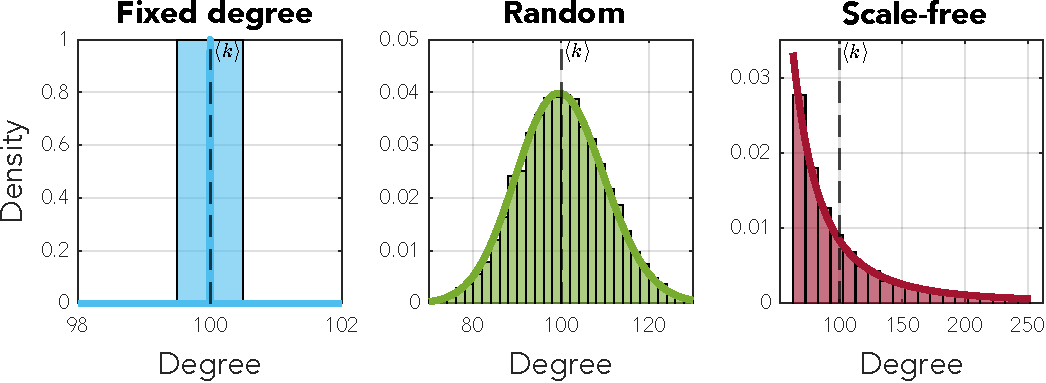
\includegraphics[width = \textwidth]{../Figures/Distributions/1D.pdf}
\caption{Univariate fixed-degree, random and scale-free distributions with the same average node degree $\kmean$ = 100. The normalised histogram of $k \in \K$ follows $P(k)$ nicely as expected. Over the course of this work the colours used to indicate the different topologies will remain constant.}
\label{fig:1Dpdfs}
\end{figure}


\subsection{Scale-free networks}
What we can often observe in nature is the preferential attachment to nodes with a high degree \cite{Bullmore2010}: the rich or famous tend to get more rich or famous. This trait is also described as the 80/20 rule by Pareto. Networks with this property consist of a small number of highly connected nodes, the \textsl{hubs}, and a large number of low degree nodes. We can represent this with a power law distribution:
\begin{align}
P(k) = C k^{-\gamma} \label{eq:scalefreepdf}
\end{align}
with $C$ a constant so that $\sum_{k=1}^{\infty} P(k) = 1$. We can also see that $C \cdot \sum_{k=1}^{\infty} k^{-\gamma} = 1$ so that $C = \sum_{k=1}^{\infty} k^{\gamma} = 1/\zeta(k)$, the Riemann Z{\`e}ta function \cite{BarabasiNetworkBook2016}. \\

To understand the scale of a distribution like \eqref{eq:scalefreepdf} we first ask ourselves how the size of the network affects the hubs. We can easily calculate the \textit{natural cutoff} $k_{\text{max}}$, the highest expected degree in the network. We only expect the largest hub to be the only hub in the domain $[k_{\text{max}}, +\infty[$:
\begin{align*}
\int_{k_{\text{max}}}^{\infty} P(k) dk=\frac{1}{N}
\end{align*}
Following \cite{BarabasiNetworkBook2016} for \eqref{eq:scalefreepdf} this results in:
\begin{align}
\kmax = \kmin \cdot N^{\frac{1}{\gamma-1}} \label{eq:scalefreecutoff}
\end{align}
So: larger networks yield larger hubs, and we can see there might be very large differences between the node degrees. In practice, it is better to choose $\kmin$ and $\kmax$ and set $P$ to zero outside of $\K$. \\



There are constraints on $\gamma$ to yield a scale-free network. When $0 < \gamma < 2$ the largest hub grows faster than $N$, so once its degree exceeds $N-1$ there are no more new nodes to connect to and the network will not be able to grow according to \eqref{eq:scalefreepdf}. A rigorous proof is given in \cite{Bassler2011}. For $\gamma = 2$, the system grows linearly, as we can see in \eqref{eq:scalefreecutoff}. When $2 < \gamma \leq 3$ we find the most scale-free networks, as for $\gamma > 3$ hubs are not sufficiently large and numerous to have much influence on the network
\cite{BarabasiNetworkBook2016}.

Networks with a distribution like \eqref{eq:scalefreepdf} are called \textit{scale-free} networks, as they lack an internal scale to represent the magnitude of the network. We can observe \eqref{eq:scalefreepdf} on different scales like the probability of two Hollywood actors appearing in a movie, or the connections between web pages on the internet \cite{Barabasi2003}.


\subsection{Networks of theta neurons}
The human brain can be seen as a graph, with neurons as graph nodes, where the pre- to postsynaptic relation models a directional edge in the network. These edges are usually unidirectional though it can happen that the post- reconnects to the presynaptic neuron. Using this knowledge, we can easily extend the model to networks of neurons:
\begin{align}
\dot{\theta}_{i} &=\left(1-\cos \theta_{i}\right)+\left(1+\cos \theta_{i}\right) \cdot \left[\eta_{i} + I_{i}(t)\right] \qquad \theta_i \in \T^N  \label{eq:thetaneuronnetwork} \\
I_{i}(t) &=\frac{\kappa}{\kmean} \sum_{j=1}^{N} A_{i j} \cdot \mathcal{P}_{n}(\theta_{j}) \label{eq:thetaneuronnetworkcurrent}
\end{align}
where the excitability $\eta_i$ allows each neuron to adjust in which regime it is situated, and $\eta_i \sim g(\eta \rvert \eta_0, \sigma)$. $\kappa$ models the macroscopic synaptic strength, and $\mathcal{P}_n(\theta)  = a_n(1 - \cos \theta)^n$ models synaptic coupling by a pulse-shaped signal, emitted when a neuron fires. As discussed in Chapter \ref{sec:Introduction}, there are conversions from the action potential to a neurotransmitter and back, but this process will be captured by using only $\mathcal{P}$ as the action potential and $\kappa$ as the "efficiency" of the conversions. $n$ models the sharpness of the pulse, and $a_n$ is a normalisation constant so that $\int_{\T} \mathcal{P}_{n} d \theta=2 \pi$. We will take $n=2$ from here, as in\cite{Luke2013, OttAntonsen2017, Martens2020}. 
%Note that for a fully connected network, $A_{ij} = 1$ so that \eqref{eq:thetaneuronnetworkcurrent} reduces to the work in \cite{Luke2013} and \cite{Martens2020}. \\

In \eqref{eq:thetaneuronnetwork} we see everything come together: changes to the phase $\theta_i$ are induced by $\dtheta_i$ which in turn depends on the bifurcation of $\theta$ with magnitude $I_i$ which depends on all neurons in the network. \\

%We can also understand why a fixed time-step solver is useful here: the memory demand of storing \eqref{eq:thetaneuronnetworkcurrent} as double precision floating point numbers is about $ \frac{t_b - t_a}{h+1} \cdot N \cdot 8 $ for $\theta$, $N^2 \cdot 8$ for $A_ij$. For 10.000 neurons integrated over 100 seconds at a time-step $h$ of 0.005 that is and 762.9 Mb respectively.

Studying a set of differential equations like \eqref{eq:thetaneuronnetworkcurrent} is not feasible, as we are quickly approaching thousands of neurons. And in the end, the dynamics of a single neuron are not of interest. Instead, we wish to capture and study how the network behaves as a whole. One aspect, synchrony, can be captured by the Kuramoto order parameter:
\begin{align}
Z(t) = \frac{1}{N} \sum_{j=1}^N e^{\ic\theta_j}  \qquad Z \in \C \label{eq:orderparameter}
\end{align}
$Z$ is a complex variable, consisting of a radius $r = \rvert Z \rvert$ and argument $\psi = \arg \left( Z \right)$, so that $Z(t) = r(t) e^{\ic \psi(t)}$. When all phases are uniformly distributed across the unit circle $\T$, then $\rvert Z \rvert = 0$, resulting in a network with no synchronisation. When all phases are exactly the same, $\rvert Z \rvert = 1$ and the network is fully scynchronised. \eqref{eq:orderparameter} describes the \textsl{mean-field} of the network, a simpler model that describes the average behaviour of the whole network. Analysis is simply conducted either on $ \rvert Z(t) \rvert$ versus time, or in the complex unit circle as $\Re (Z(t))$ versus $\Im (Z(t))$.

Different works on the dynamics of \eqref{eq:orderparameter} have been published \cite{Luke2013, Martens2020}, and we will build on that analysis in the following chapters.


